\chapter{相关理论与技术基础}
\label{chp:foundations}

本章旨在为后文提出的机器人自主操作算法提供必要的理论支撑与技术背景。内容将围绕机器人模仿学习这一核心技术路线展开，系统性地介绍其研究所需的前置知识。首先，将对机械臂运动学与控制的基本原理进行阐述，重点介绍 Denavit-Hartenberg 参数法在运动学建模中的应用，为后续的动作生成提供物理约束与数学基础。随后，将介绍模仿学习理论，探讨其基本原理以及当前典型的模仿学习算法。最后，将介绍视觉语言动作模型的核心思想与结构原理，它构成了本文所提算法的基石。

\section{机械臂运动学建模}
\label{sec:kinematics}

机械臂运动学是研究机械臂在空间中的运动特性而不考虑其受力的学科，其核心任务是建立机械臂各关节变量与末端执行器在笛卡尔空间中位姿之间的数学关系。这种关系是实现机械臂运动控制以及与环境交互的基础。本节将遵循“理论-方法-应用”的逻辑层次，首先介绍基于标准D-H参数的运动学建模理论，随后阐述正向与逆向运动学的一般求解方法，最后将该理论与方法应用于本研究所涉及的具体机械臂，给出其运动学模型的详细求解过程。

\subsection{基于标准D-H参数的运动学建模}
\label{subsec:dh_modeling}

为描述机械臂上各个连杆的位置和姿态，需要在机械臂的关键位置上固连一系列的坐标系，例如基坐标系 \{B\}、工具坐标系 \{T\} 以及每个连杆的连杆坐标系 \{i\}。不同坐标系之间的相对位姿关系可以通过齐次变换矩阵进行描述。一个通用的齐次变换矩阵 $T$ 是一个 $4 \times 4$ 的矩阵，其形式如式\ref{eq:homogeneous_transform}所示。

\begin{equation}
  \label{eq:homogeneous_transform}
  T = \begin{bmatrix}
    R & p \\
    0 & 1
  \end{bmatrix} = \begin{bmatrix}
    n_x & o_x & a_x & p_x \\
    n_y & o_y & a_y & p_y \\
    n_z & o_z & a_z & p_z \\
    0 & 0 & 0 & 1
  \end{bmatrix}
\end{equation}

其中，$R \in SO(3)$ 是一个 $3 \times 3$ 的旋转矩阵，用于描述坐标系之间的相对姿态；$p \in \mathbb{R}^3$ 是一个 $3 \times 1$ 的平移向量，用于描述坐标系原点之间的相对位置。通过齐次变换矩阵，可以实现坐标点在不同坐标系下的表示转换以及多级坐标变换的复合运算。

Denavit-Hartenberg 参数法是一种建立机械臂各连杆坐标系并描述其相对位姿的标准方法，如图\ref{fig:dh_parameters}所示，它仅用四个参数即可唯一确定两个相邻连杆坐标系之间的几何关系。这四个参数，即连杆长度 $a_{i-1}$、连杆扭转角 $\alpha_{i-1}$、连杆偏距 $d_i$ 和关节角 $\theta_i$，其定义如表\ref{tab:dh_parameters}所示。

\begin{figure}[htbp]
  \centering
  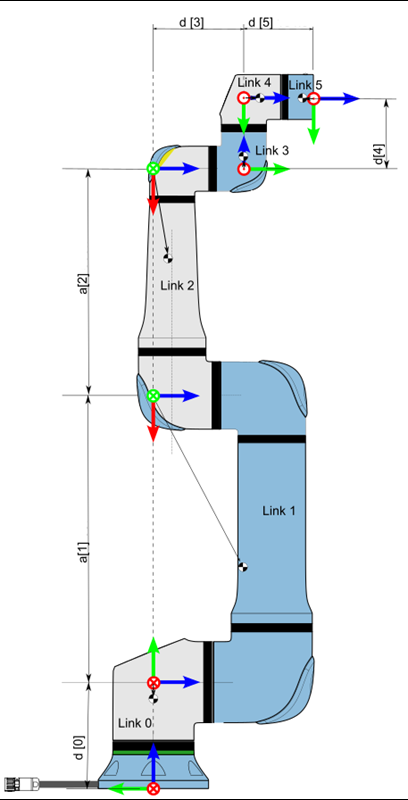
\includegraphics[width=0.4\textwidth]{figures/content/ur-dhmodel.png}
  \caption{D-H参数定义示意图}
  \label{fig:dh_parameters}
\end{figure}

\begin{table}[htbp]
  \centering
  \caption{标准D-H参数定义}
  \label{tab:dh_parameters}
  \begin{tabular}{cl}
    \toprule
    参数 & 定义 \\
    \midrule
    $a_{i-1}$ & 沿 $x_{i-1}$ 轴，从 $z_{i-1}$ 移动到 $z_i$ 的距离 \\
    $\alpha_{i-1}$ & 绕 $x_{i-1}$ 轴，从 $z_{i-1}$ 旋转到 $z_i$ 的角度 \\
    $d_i$ & 沿 $z_i$ 轴，从 $x_{i-1}$ 移动到 $x_i$ 的距离 \\
    $\theta_i$ & 绕 $z_i$ 轴，从 $x_{i-1}$ 旋转到 $x_i$ 的角度 \\
    \bottomrule
  \end{tabular}
\end{table}

根据D-H参数的定义，从坐标系\{i-1\}到坐标系\{i\}的变换可以分解为四次基本变换的乘积，其对应的齐次变换矩阵 $A_i$ 如式\ref{eq:dh_transform}所示。

\begin{equation}
  \label{eq:dh_transform}
  \begin{aligned}
    A_i &= \text{Rot}_{z, \theta_i} \text{Trans}_{z, d_i} \text{Trans}_{x, a_{i-1}} \text{Rot}_{x, \alpha_{i-1}} \\
        &= \begin{bmatrix}
          \cos\theta_i & -\sin\theta_i\cos\alpha_{i-1} & \sin\theta_i\sin\alpha_{i-1} & a_{i-1}\cos\theta_i \\
          \sin\theta_i & \cos\theta_i\cos\alpha_{i-1} & -\cos\theta_i\sin\alpha_{i-1} & a_{i-1}\sin\theta_i \\
          0 & \sin\alpha_{i-1} & \cos\alpha_{i-1} & d_i \\
          0 & 0 & 0 & 1
        \end{bmatrix}
  \end{aligned}
\end{equation}

通过为机械臂的每个连杆建立D-H参数表，即可得到从 $i=1$ 到 $n$ 的所有变换矩阵 $A_i$，为后续的正向与逆向运动学求解奠定数学基础。

\subsection{机械臂正逆向运动学求解}
\label{subsec:fk_ik_solution}

运动学求解旨在建立关节空间与笛卡尔空间之间的映射关系，是实现机械臂控制的核心。本小节将分别介绍正向运动学与逆向运动学求解的通用方法，为后续针对具体机械臂的分析提供理论框架。

正向运动学旨在根据已知的机械臂各关节变量，计算出末端执行器相对于基坐标系的位姿。通过D-H参数法建立的各连杆变换矩阵，这一过程可以通过将从基座到末端的连续变换矩阵 $A_i$ 依次相乘得到。对于一个 $n$ 自由度的机械臂，其末端执行器坐标系 \{n\} 相对于基坐标系 \{0\} 的总变换矩阵 $T_n^0$ 可由式\ref{eq:forward_kinematics}计算得出。

\begin{equation}
  \label{eq:forward_kinematics}
  T_n^0 = A_1(\theta_1) A_2(\theta_2) \cdots A_n(\theta_n)
\end{equation}

最终得到的 $T_n^0$ 矩阵中的旋转部分和平移部分即分别对应末端执行器的姿态和位置。正向运动学模型是唯一的，即一组给定的关节变量只能对应一个确定的末端位姿。

逆向运动学是正向运动学的逆问题，即根据给定的末端执行器在笛卡尔空间中的期望位姿，反向求解出满足该位姿的一组或多组关节变量。与正向运动学不同，逆向运动学的求解过程更为复杂，其解可能不唯一、存在多组解，或者在机械臂工作空间之外无解。逆向运动学的求解方法主要分为解析法和数值法两类。

解析法，也称代数法或几何法，通过对方程组 $T_n^0$ 进行代数运算或利用机械臂的几何关系来直接求解关节变量的封闭解。该方法计算速度快、能够求出所有可能的解，但仅适用于结构相对简单的机械臂，例如具有球形腕关节的六自由度机械臂。对于结构复杂的冗余机械臂，解析法通常难以适用。

数值法是一种迭代求解方法，它将逆向运动学问题转化为一个非线性优化问题。该方法从一个初始的关节角配置出发，通过迭代计算来逐步减小当前末端位姿与期望位姿之间的误差，直至误差小于预设阈值。基于雅可比矩阵的迭代法是其中最常用的一种，其核心思想如式\ref{eq:jacobian_inverse}所示。

\begin{equation}
  \label{eq:jacobian_inverse}
  \Delta\theta = J^{-1} \Delta x
\end{equation}

其中，$\Delta x$ 是末端位姿误差，$\Delta\theta$ 是关节角度的修正量，$J$ 是描述末端执行器速度与关节速度之间线性关系的雅可比矩阵。数值法通用性强，适用于任意结构的机械臂，但其计算量较大，可能陷入局部最优，且解的精度和收敛速度依赖于初始值的选取和迭代算法的设计。

\subsection{具体机械臂运动学求解}
\label{subsec:specific_robot_kinematics}

本节将前述理论应用于本研究后续实验所采用的 Franka Emika Panda 与 Universal Robots UR5 两款机械臂，对其运动学模型进行具体分析与求解。

Franka Emika Panda 是一款七自由度的冗余机械臂，其结构紧凑、灵活性高，广泛应用于学术研究。本研究的仿真实验将基于该款机械臂展开。根据其官方文档及相关研究，其改进D-H参数如表\ref{tab:panda_dh_parameters}所示。

\begin{table}[htbp]
  \centering
  \caption{Franka Panda 机械臂改进D-H参数}
  \label{tab:panda_dh_parameters}
  \begin{tabular}{ccccc}
    \toprule
    关节 $i$ & 连杆扭转角 $\alpha_{i-1}$ (rad) & 连杆长度 $a_{i-1}$ (m) & 连杆偏距 $d_i$ (m) & 关节角 $\theta_i$ (rad) \\
    \midrule
    1 & 0 & 0 & 0.333 & $\theta_1$ \\
    2 & $-\pi/2$ & 0 & 0 & $\theta_2$ \\
    3 & $\pi/2$ & 0 & 0.316 & $\theta_3$ \\
    4 & $\pi/2$ & 0.0825 & 0 & $\theta_4$ \\
    5 & $-\pi/2$ & -0.0825 & 0.384 & $\theta_5$ \\
    6 & $\pi/2$ & 0 & 0 & $\theta_6$ \\
    7 & $\pi/2$ & 0.088 & 0.107 & $\theta_7$ \\
    \bottomrule
  \end{tabular}
\end{table}

将表\ref{tab:panda_dh_parameters}中的参数代入式\ref{eq:dh_transform}，即可得到各关节的变换矩阵 $A_i$。例如，前两个关节的变换矩阵如式\ref{eq:panda_A1A2}所示。

\begin{equation}
\label{eq:panda_A1A2}
\begin{aligned}
A_1 &= \begin{bmatrix} c_1 & -s_1 & 0 & 0 \\ s_1 & c_1 & 0 & 0 \\ 0 & 0 & 1 & d_1 \\ 0 & 0 & 0 & 1 \end{bmatrix}, \quad
A_2 = \begin{bmatrix} c_2 & 0 & -s_2 & 0 \\ s_2 & 0 & c_2 & 0 \\ 0 & -1 & 0 & 0 \\ 0 & 0 & 0 & 1 \end{bmatrix}
\end{aligned}
\end{equation}

其中 $c_i = \cos\theta_i, s_i = \sin\theta_i$。其余各关节变换矩阵可同理求得。将所有变换矩阵连乘即可得到其正向运动学解 $T_7^0 = A_1 A_2 A_3 A_4 A_5 A_6 A_7$。由于 Franka Panda 是七自由度冗余机械臂，其逆运动学不存在封闭解析解，通常采用基于雅可比矩阵的数值法进行求解，利用其冗余自由度来优化关节限制、避开奇异点或执行次级任务。


Universal Robots UR5 是一款经典的六自由度协作机械臂，本研究的实物实验平台将采用该款机械臂。根据其官方文档，其标准D-H参数如表\ref{tab:ur5_dh_parameters}所示。

\begin{table}[htbp]
  \centering
  \caption{UR5 机械臂标准D-H参数}
  \label{tab:ur5_dh_parameters}
  \begin{tabular}{ccccc}
    \toprule
    关节 $i$ & 连杆扭转角 $\alpha_{i-1}$ (rad) & 连杆长度 $a_{i-1}$ (m) & 连杆偏距 $d_i$ (m) & 关节角 $\theta_i$ (rad) \\
    \midrule
    1 & $\pi/2$ & 0 & 0.089159 & $\theta_1$ \\
    2 & 0 & -0.42500 & 0 & $\theta_2$ \\
    3 & 0 & -0.39225 & 0 & $\theta_3$ \\
    4 & $\pi/2$ & 0 & 0.10915 & $\theta_4$ \\
    5 & $-\pi/2$ & 0 & 0.09465 & $\theta_5$ \\
    6 & 0 & 0 & 0.08230 & $\theta_6$ \\
    \bottomrule
  \end{tabular}
\end{table}

UR5 机械臂的腕部三轴交于一点，满足 Pieper 准则，因此其逆运动学存在封闭的解析解。求解过程采用解析法，通过解耦思想将位置和姿态问题分开处理。该方法首先通过求解腕部中心点的位置来确定前三个关节 $\theta_1, \theta_2, \theta_3$ 的值，随后基于已求出的前三个关节的姿态来解算后三个腕部关节 $\theta_4, \theta_5, \theta_6$。具体推导过程如下：

给定末端期望位姿矩阵 $T_6^0 = \begin{bmatrix} R & p \\ 0 & 1 \end{bmatrix} = \begin{bmatrix} n_x & o_x & a_x & p_x \\ n_y & o_y & a_y & p_y \\ n_z & o_z & a_z & p_z \\ 0 & 0 & 0 & 1 \end{bmatrix}$，腕部中心点 $p_c$ 的位置可以通过从末端点 $p$ 沿末端坐标系 $z_6$ 轴的反方向平移 $d_6$ 得到：

\begin{equation}
  p_c = p - d_6 \cdot R \cdot \begin{bmatrix} 0 \\ 0 \\ 1 \end{bmatrix} = \begin{bmatrix} p_x - d_6 a_x \\ p_y - d_6 a_y \\ p_z - d_6 a_z \end{bmatrix}
\end{equation}

关节角 $\theta_1$ 的求解涉及到将 $p_c$ 投影到 $x_0-y_0$ 平面。从俯视角度看，$p_c$ 的投影点、基座原点以及关节2的轴线构成一个三角形，通过反正切函数和余弦定理即可求解。$\theta_1$ 通常存在两组解，对应机械臂左手和右手两种不同的构型：

\begin{equation}
  \theta_1 = \text{arctan2}(p_{cy}, p_{cx}) - \text{arctan2}(d_4, \pm\sqrt{p_{cx}^2 + p_{cy}^2 - d_4^2})
\end{equation}

关节角 $\theta_5$ 的求解利用了变换矩阵的特性。将总变换方程 $T_6^0 = T_1^0 T_2^1 T_3^2 T_4^3 T_5^4 T_6^5$ 左乘 $(T_1^0)^{-1}$，得到 $T_6^1 = (T_1^0)^{-1} T_6^0$。展开该矩阵的对应元素，可以发现它仅与 $\theta_5$ 有关，从而得到 $\theta_5$ 的两组解：

\begin{equation}
  \theta_5 = \pm \text{arccos}\left(\frac{p_x s_1 - p_y c_1 - d_4}{d_6}\right)
\end{equation}

关节角 $\theta_6$ 可在求出 $\theta_5$ 后，通过 $T_6^1$ 矩阵的旋转部分元素得到。当 $\sin\theta_5 \neq 0$ 时，即非奇异位形下：

\begin{equation}
  \theta_6 = \text{arctan2}\left(\frac{-o_x s_1 + o_y c_1}{\sin\theta_5}, \frac{n_x s_1 - n_y c_1}{\sin\theta_5}\right)
\end{equation}

关节角 $\theta_3$ 的求解同样利用几何关系。在关节2和关节3所在的平面内，连杆 $a_2$ 和 $a_3$ 与 $p_c$ 在该平面上的投影构成一个三角形。利用余弦定理可得：

\begin{equation}
  \theta_3 = \pm \text{arccos}\left(\frac{\|p_{c}\|^2 - d_1^2 - d_4^2 - a_2^2 - a_3^2}{2 a_2 a_3}\right)
\end{equation}

关节角 $\theta_2$ 可由 $\theta_1$ 和 $\theta_3$ 共同确定。其求解涉及到求解一个关于 $\sin\theta_2$ 和 $\cos\theta_2$ 的线性方程组，最终可表示为：

\begin{equation}
  \theta_2 = \text{arctan2}(-p_{cz}, \pm\sqrt{p_{cx}^2+p_{cy}^2-d_4^2}) - \text{arctan2}(a_3 s_3, a_2 + a_3 c_3)
\end{equation}

最后，关节角 $\theta_4$ 可由旋转矩阵 $R_3^6 = (R_3^0)^{-1} R_6^0$ 的元素得到，其中 $R_3^0$ 由已求出的前三个关节角确定：

\begin{equation}
  \theta_4 = \text{arctan2}(R_{3,2}^6, R_{3,1}^6)
\end{equation}

由于三角函数的周期性和对称性，UR5 的逆运动学通常存在八组不同的关节角配置，均能使末端达到同一位姿。该解析解能够计算出所有可能的关节角配置，为实时控制提供了确定性的解集。

\section{模仿学习理论}
\label{sec:imitation_learning}

\subsection{模仿学习原理}
\label{subsec:il_principles}

模仿学习的核心目标是让智能体通过观察专家的示范数据，隐式地学习并内化专家的行为策略，从而使其在面对相似的状态与场景时，能够自主做出与专家一致的决策。与高度依赖奖励函数工程和大量试错探索的强化学习相比，模仿学习能够更自然、更高效地从人类直觉操作中提取高维任务特征，极大降低了策略学习的样本复杂度与安全风险。

在模仿学习的理论框架中，机械臂与环境的交互过程通常被建模为离散时间的部分可观察马尔可夫决策过程。该过程可以用一个多元组 $\mathcal{M} = \langle \mathcal{S}, \mathcal{A}, \mathcal{P}, \mathcal{R}, \Omega, \mathcal{O}, \gamma, \rho_0 \rangle$ 来进行形式化定义。具体而言，$\mathcal{S}$ 表示系统的真实状态空间，在机械臂任务中通常包含机械臂各关节的绝对角度、末端执行器的物理开合状态以及环境中物体的真实位姿；$\mathcal{A}$ 表示动作空间，定义了智能体能够执行的连续控制指令集合，例如关节的角速度或轴角目标位置；$\mathcal{P}(s_{t+1}|s_t, a_t)$ 是环境的状态转移概率分布，描述了在状态 $s_t$ 下执行动作 $a_t$ 后系统状态演化的动力学机制。由于传感器噪声和视觉遮挡，机械臂无法获取完整的真实状态，只能获得观测空间 $\Omega$ 中的观测值 $o_t$，这一过程由观测概率分布 $\mathcal{O}(o_t|s_t)$ 决定。$\mathcal{R}(s_t, a_t)$ 为潜在的真实奖励函数，而模仿学习的根本特征即在于不依赖与环境交互来获取此显式奖励；$\gamma$ 为折扣因子，$\rho_0(s_1)$ 则是初始状态分布。

在标准设定中，假定存在一个具有极高任务完成率的专家策略，表示为条件概率分布 $\pi_E(a|s)$。在训练阶段，算法接收一组由专家提供的演示轨迹集合 $\mathcal{D} = \{\tau_1, \tau_2, \dots, \tau_N\}$。其中，每一条轨迹 $\tau_i$ 记录了从初始状态到终止状态的完整序列交互，可表示为 $\tau_i = \{(o_1, a_1), (o_2, a_2), \dots, (o_T, a_T)\}$。模仿学习的最终目的，是在给定的参数化策略空间中，寻找一个由神经网络参数化的最优策略 $\pi_\theta(a|o)$，使其最大程度地逼近专家策略。

传统行为克隆是模仿学习中最基础且应用最为广泛的方法。它将序列决策学习过程直接转化为一个标准的监督学习问题，摒弃了对时间依赖性和环境动力学的假设。在概率论视角下，行为克隆的目标是最大化专家演示数据在参数化策略下的对数似然期望。其优化目标可表述为：

\begin{equation}
  \theta^* = \arg\max_\theta \mathbb{E}_{(o,a) \sim \mathcal{D}} \left[ \log \pi_\theta(a|o) \right]
\end{equation}

在实际的机械臂连续控制任务中，动作空间是连续且高维的。若假设学习到的策略服从各向同性的高斯分布，即 $\pi_\theta(a|o) = \mathcal{N}(\mu_\theta(o), \Sigma)$，其中均值 $\mu_\theta(o)$ 由深度神经网络输出，$\Sigma = \sigma^2 I$ 为固定的协方差矩阵。根据高斯分布的概率密度函数，最大化对数似然目标可以等价转换为最小化网络预测动作与专家真实动作之间的均方误差：

\begin{equation}
  \mathcal{L}_{\text{BC}}(\theta) = \frac{1}{|\mathcal{D}|} \sum_{(o,a) \in \mathcal{D}} \| a - \mu_\theta(o) \|^2
\end{equation}

尽管行为克隆凭借其算法实现上的简单性与直接性，在诸多视觉控制任务中取得了初步成功，但其独立同分布的强假设在马尔可夫决策过程中是失效的。当机械臂根据当前学习到的策略在物理环境中实际执行动作时，其当前时刻微小的预测误差会不可避免地改变下一时刻的环境状态，从而破坏了测试时状态分布与训练时专家状态分布的一致性。这种由微小误差引发的连锁反应，正是限制行为克隆在复杂任务中应用的核心理论瓶颈。为了突破这一瓶颈，近期的研究转向利用长序列依赖建模和动作空间扩展，通过从根本上改变动作预测的时域结构来延缓甚至消除这种误差累积。
\subsection{典型模仿学习算法}
\label{subsec:typical_il_algorithms}

在解决精细操作任务的模仿学习问题时，动作分块 Transformer 算法（Action Chunking with Transformers, ACT）\cite{zhao2023learning} 表现出了优异的性能。该算法基于 Transformer 架构构建了条件变分自编码器的编码器和解码器，用于对示教数据进行建模。具体而言，编码器负责对输入数据进行处理并高效提取关键特征；解码器则先借助 ResNet 网络对图像进行编码，随后通过 Transformer 编码器将多模态特征深度融合，最终由 Transformer 解码器生成连贯、流畅的动作序列。

针对模仿学习中存在的误差累积和人类演示非平稳问题，ACT 采用了动作分块策略。该策略将连续的动作序列分割为多个相对独立的动作组块，有效减少了误差在动作执行过程中的传递与积累。在面对高精度控制和闭环反馈的精细操作任务时，ACT 策略会预测未来 $k$ 个时间步的动作，使得任务的有效视野降低 $k$ 倍，以此缓解误差累积问题。

此外，为提升策略的平滑性，ACT 引入了时间集成机制。在每个时间步推理动作序列时，生成不同时刻的动作组块，并按时序排列使不同动作组块相互重叠。在任一时间步生成多个预测动作后，采用指数加权平均的方式组合这些预测：

\begin{equation}
  w_i = \exp(-m \cdot i)
\end{equation}

其中 $w_0$ 是初始动作的权重，$m$ 为权重系数。这种加权组合机制进一步优化了动作生成的连贯性。

% \begin{figure}[htbp]
%   \centering
%   \includegraphics[width=0.6\textwidth]{figures/content/[此处需要补充具体数据/文献/细节]}
%   \caption{基于 Transformer 的 ACT 模仿学习框架}
%   \label{fig:act_architecture}
% \end{figure}

尽管 ACT 算法在精细操作任务中成效显著，但其在处理复杂动作分布和高维动作空间能力上仍有不足，难以执行复杂手部动作。相比之下，扩散策略算法（Diffusion Policy）\cite{chi2023diffusion} 能够在处理复杂动作分布时精准生成合适策略，高效探索高维动作空间并寻得最优解，且具备出色的训练稳定性。

扩散策略基于去噪扩散概率模型，以随机朗之万动力学为理论基础，将动作序列的生成视为去噪过程。传统的显式策略将世界状态直接映射到动作，在处理多模态行为时存在局限；隐式策略通过能量函数定义动作分布，虽能表示多模态分布但训练时需负采样导致过程不稳定。扩散策略则不直接输出动作，而是基于视觉观察推断动作分数的梯度，并通过迭代逐步优化动作。这使其能够自然精确地表达多模态动作分布，适应高维动作空间，并通过直接学习能量函数梯度避免了传统负采样的不稳定问题。

在具体原理上，扩散策略的输出生成过程被建模为去噪过程。在第 $k$ 次迭代中，去噪公式如下：

\begin{equation}
  x^{k-1} = \alpha \left( x^k - \gamma \epsilon_\theta(x^k, k) + \mathcal{N}(0, \sigma^2 I) \right)
\end{equation}

其中，$\epsilon_\theta(x^k, k)$ 是噪声预测网络，通过学习不断优化以准确预测噪声；$\alpha$、$\gamma$ 和 $\sigma$ 是与迭代步骤 $k$ 相关的参数，共同构成噪声调度；$\mathcal{N}(0, \sigma^2 I)$ 是每次迭代添加的高斯噪声，为迭代引入随机性以避免陷入局部最优。训练时，通过最小化均方误差损失函数来训练噪声预测网络：

\begin{equation}
  L = \text{MSE} \left( \epsilon^k, \epsilon_\theta(x^0 + \epsilon^k, k) \right)
\end{equation}

为适应机械臂任务，扩散策略在视觉观察条件设定方面进行了改进，使用扩散模型近似条件分布以加快扩散过程。给定时间步 $t$ 的观察数据 $O_t$，预测动作序列 $A_t$ 的去噪过程具体为：

\begin{equation}
  A_t^{k-1} = \alpha \left( A_t^k - \gamma \epsilon_\theta(O_t, A_t^k, k) + \mathcal{N}(0, \sigma^2 I) \right)
\end{equation}

相应的训练损失公式为：

\begin{equation}
  L = \text{MSE} \left( \epsilon^k, \epsilon_\theta(O_t, A_t^0 + \epsilon^k, k) \right)
\end{equation}

% \begin{figure}[htbp]
%   \centering
%   \includegraphics[width=0.6\textwidth]{figures/content/[此处需要补充具体数据/文献/细节]}
%   \caption{不同策略表示方法对比及 Diffusion Policy 算法框架}
%   \label{fig:diffusion_policy_architecture}
% \end{figure}

在闭环动作序列预测上，扩散策略将动作序列预测能力与滚动时域控制相结合。在时间步 $t$，以最近 $T_o$ 步的观察数据为输入，预测 $T_p$ 步的动作，其中前 $T_a$ 步的动作会被直接执行在机械臂上而无需重新规划。这种设计平衡了长期规划与实时响应。

在网络架构设计上，扩散策略采用 CNN 和 Transformer 架构进行构建。基于 CNN 的架构使用修改后的 1D 时间卷积网络，借助 FiLM 预测动作轨迹；基于 Transformer 的架构则凭借输入与注意力机制，在高复杂度任务中表现卓越。具体而言，采用 ResNet18 作为视觉编码器，以空间 Softmax 池化替换全局平均池化以保留图像空间信息；用 GroupNorm 替代 BatchNorm 并与指数移动平均相结合，有效保障了训练稳定性。通过噪声调度合理调控扩散过程中的噪声变化，助力模型捕捉动作信号的高频和低频特征，从而优化动作生成的准确性与稳定性。

\section{视觉语言动作模型}
\label{sec:vla_models}

[此处需要补充视觉语言动作模型相关内容]
